% ! TeX root = ../bachelor-thesis.tex

\chapter{Definizione del problema}
\label{ch:Chapter1}

In questo capitolo, sarà introdotto lo scopo del progetto e saranno illustrati
i concetti fondamentali che consentiranno al lettore di comprendere a pieno
l’obiettivo del progetto e le tecnologie utilizzate per realizzarlo.

\section{Scopo del progetto}
\label{sec:Sezione1.1}

Questo progetto nasce con lo scopo di assistere persone anziane, fragili o con
disabilità, permettendo loro di ottenere una certa indipendenza nello svolgere
le azioni quotidiane in ambito domestico. Inoltre, si propone di fornire un
servizio integrativo per poter mantenere in allenamento le proprie capacità
cognitive. Questo servizio potrà essere utilizzato anche in un contesto
socio-sanitario, dagli operatori competenti, per realizzare un percorso
educativo per pazienti con difficoltà cognitive e monitorarne i progressi, così
da tenere traccia dei miglioramenti ottenuti.

L’idea è quella d'integrare un’assistente vocale a un sistema domotico, creando
una suite che comprenderà i servizi di entrambi. Nello specifico, il
\textit{sistema domotico} si occuperà di agevolare la vita domestica degli
utenti, rendendo più accessibili gli strumenti di uso quotidiano, come porte e
finestre. L’\textit{assistente vocale} fornirà invece un supporto al sistema
domotico, permettendo di controllarlo tramite comandi vocali, ma consentirà
anche di accedere agli esercizi cognitivi di cui è composto il servizio
integrativo, che si baserà perciò su interazioni prettamente vocali. Per gli
esercizi cognitivi, si è pensato di progettare dei giochi che richiedano
l’impiego di alcune funzioni cognitive del cervello, seguendo i principi di
\textit{gamification}. In questo modo, si rende il servizio più accattivante,
stimolando l'utente all'utilizzo dello stesso.

\section{Contesto}
\label{sec:Sezione1.2}

Di seguito sarà contestualizzato il progetto, approfondendo i concetti che sono
stati utilizzati per descriverlo.

In particolare, si introdurrà la domotica, distinguendo il concetto d'impianto
domotico da quello di \textit{smart home} e descrivendo alcuni degli approcci
usati per controllare un sistema domotico. Seguirà poi, una breve storia sullo
sviluppo degli assistenti vocali e delle funzioni che ricoprono oggigiorno.
Infine, saranno illustrate le capacità cognitive del cervello, in modo da poter
comprendere come il servizio che si vuole progettare possa esercitarle, dunque
mantenendole in allenamento.

\subsection{La domotica}
\label{subsec:Sezione1.2.1}

Il termine \textit{domotica} \cite{DOMOTIC_SYSTEM} deriva dal latino
\textit{domus}, ovvero \textit{casa}, e dal suffisso greco \textit{-ticos}, che
indica le discipline che si applicano a un determinato concetto. Nello
specifico, il termine indica la scienza che studia e applica delle tecnologie
adatte a migliorare la qualità della vita in ambiente domestico.

L’applicazione della domotica si manifesta spesso sotto forma di un impianto
domotico. Un impianto domotico è l’insieme composto da alcuni dispositivi
elettronici e dell’infrastruttura che questi utilizzano per comunicare tra di
loro (un esempio, è l’impianto \textit{KNX} \cite{KONNEX}). Un dispositivo
domotico è infatti uno strumento non più solo passivo, ovvero che subisce
solamente le sollecitazioni dall’ambiente esterno, ma ha anche una parte
attiva, che processa tali sollecitazioni e le trasmette come eventi
identificabili e recepibili da altri strumenti. In questo modo, si crea un
organismo di strumenti che producono eventi e che possono reagire ad alcuni di
essi, modificando lo stato in cui si trovano.

I costi di un impianto domotico sono piuttosto ingenti e dipendono in parte dai
dispositivi da acquistare, ma soprattutto dalla progettazione e installazione
dell’infrastruttura su cui comunicheranno. Per questo, oggi la domotica si
manifesta molto più comunemente sotto forma di \textbf{\textit{smart home}}
(Figura \ref{fig:figure1.1}). Una \textit{smart home} è simile a un impianto
domotico, ma non necessita dell’installazione di un’infrastruttura ad hoc,
infatti ne utilizza una preesistente: Internet. I dispositivi che ricevono e
trasmettono eventi attraverso una connessione a Internet prendono il nome di
dispositivi smart, e sono alla base dell’\textbf{\textit{Internet Of Things}}.

\begin{figure}[!ht]
  \centering
  \includegraphics[scale=0.30]{resources/images/other/smart-home-example.png}
  \caption{
    L'idea di \textit{smart home}: tutti i dispositivi domestici sono connessi
    tra loro tramite Internet e possono essere controllati da remoto.
  }
  \label{fig:figure1.1}
\end{figure}

Normalmente, il controllo di questi dispositivi è affidato ad applicazioni
particolari, magari legate a uno specifico produttore. Queste prediligono un
setup facile e veloce, consentendo a chiunque di domotizzare la propria casa
senza troppe difficoltà e di controllarla generalmente tramite cellulare (ad
esempio, \textit{Philips Hue} \cite{PHILIPS}). Tuttavia, questi sistemi sono
spesso vincolati ai dispositivi di uno specifico produttore.

Quando alla \textit{smart home} si integrano dispositivi anche molto diversi
tra loro o addirittura incompatibili, diventa invece necessario un sistema di
controllo centralizzato. Solitamente, questi sistemi richiedono un setup
complesso e delle conoscenze abbastanza approfondite in materia, ma permettono
d'intermediare le interazioni tra i dispositivi, di controllarli molto più
liberamente e di creare delle regole di automazione più complesse (ad esempio,
\textit{OpenHAB} \cite{OPENHAB}).

Un altro dei vantaggi di una \textit{smart home} è la possibile integrazione
con un’assistente vocale: una tecnologia che consente d'interagire con il
proprio sistema domotico attraverso comandi vocali e di dare una voce ai propri
strumenti.

\subsection{Gli assistenti vocali}
\label{subsec:Sezione1.2.2}

Gli \textit{assistenti vocali} sono una tecnologia che si è diffusa
recentemente, il cui sviluppo risale tuttavia già al 1952, con il primo
dispositivo in grado di riconoscere delle cifre decimali in linguaggio parlato:
\textit{Audrey} di \textit{Bell Labs}. Dieci anni più tardi, fu \textit{IBM} a
proporre \textit{Shoebox}, il primo calcolatore in grado di riconoscere
operazioni matematiche in linguaggio parlato. Così, dagli anni '70 lo studio
degli assistenti vocali iniziò a diffondersi, fino a portare i risultati
odierni. \cite{VOCAL_ASSISTANT}

Oggi un’assistente vocale è uno strumento che permette d'interagire con dei
servizi attraverso dei comandi vocali. Nello specifico, è esso stesso un
servizio, basato sull’intelligenza artificiale e il \textit{machine learning},
capace di tradurre il linguaggio parlato in dati comprensibili a una macchina
(\textit{STT: Speech To Text}) e viceversa (\textit{TTS: Text To Speech}), così
proponendosi come ottimo intermediario nelle interazioni tra le persone e le
macchine.

Normalmente, si interagisce con un’assistente vocale tramite cellulare,
computer o tramite un apposito dispositivo del produttore specifico. Queste
però sono solo interfacce, infatti si occupano solo di registrare le richieste
dell’utente, per poi inviare le registrazioni al servizio vero e proprio per
essere interpretate. Tale servizio è solitamente installato su un
\textit{cloud}, ovvero su un insieme di cluster di macchine in remoto.

\begin{figure}[!ht]
  \centering
  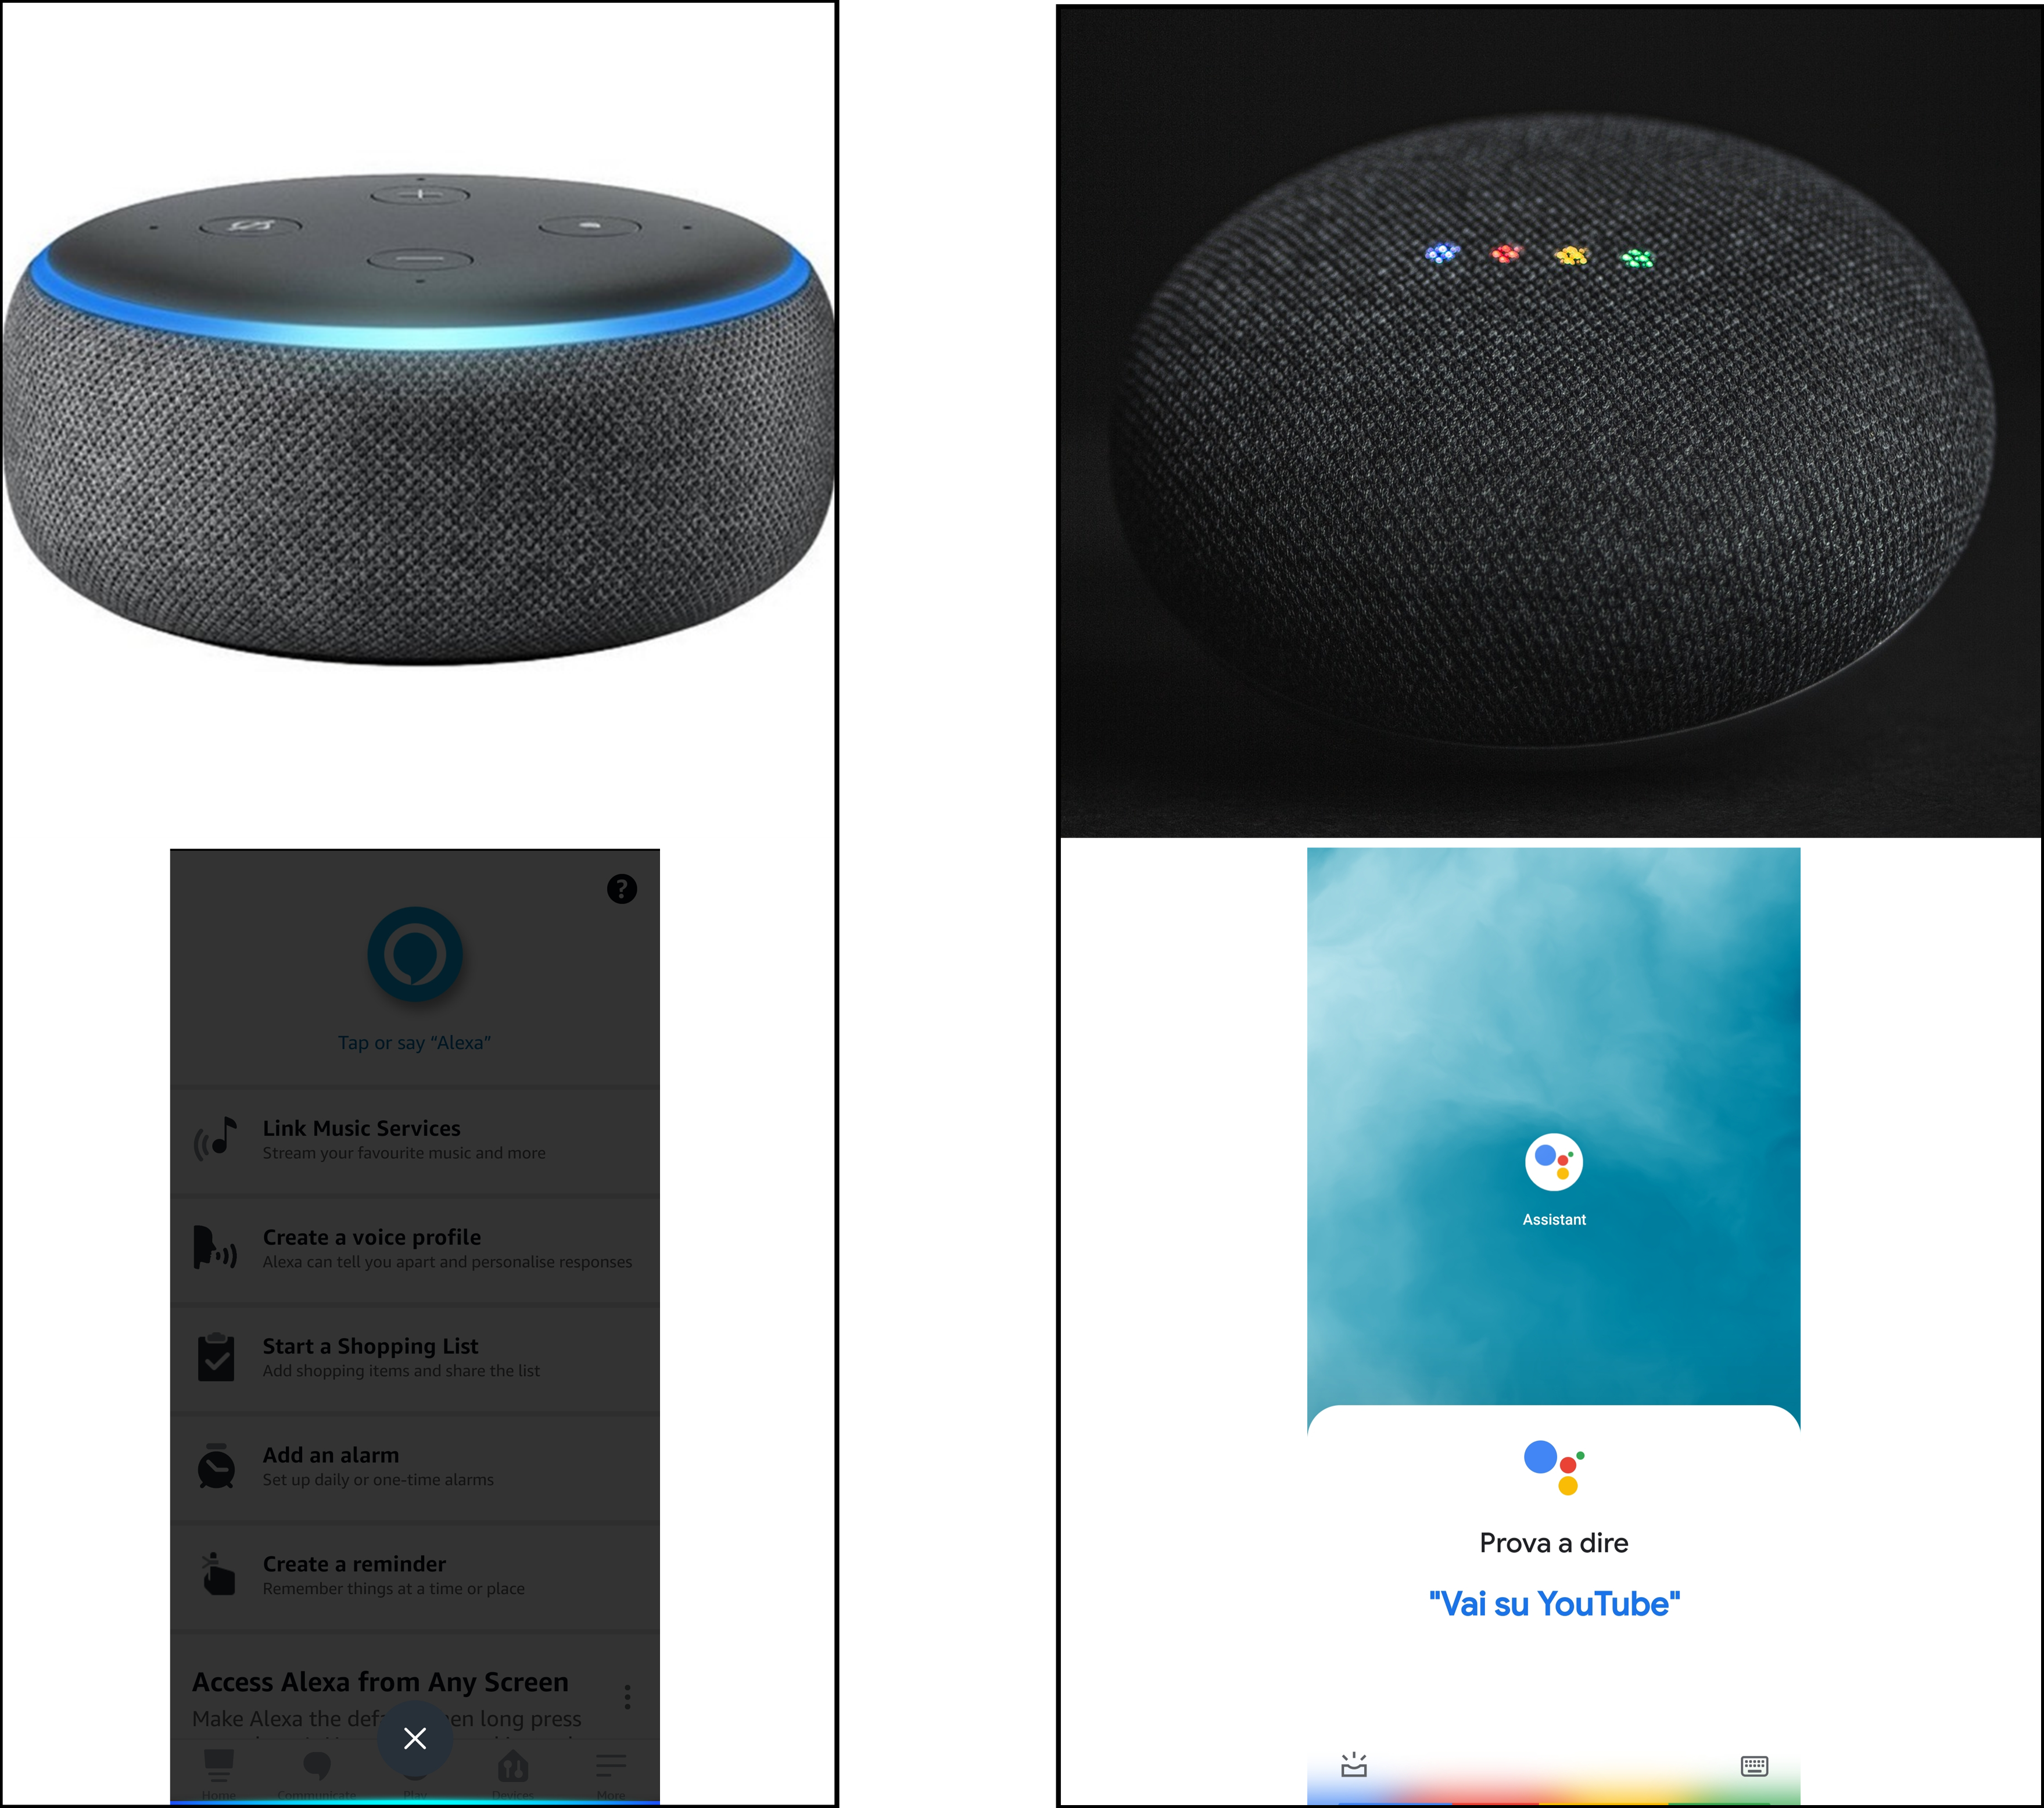
\includegraphics[scale=0.19]{resources/images/other/alexa-and-google-assistant.png}
  \caption{
    Alcuni degli assistenti vocali più conosciuti insieme alla loro
    applicazione per cellulare: a sinistra, \textit{Alexa} di Amazon; a destra,
    \textit{Google Assistant} di Google.
  }
  \label{fig:figure1.2}
\end{figure}

Gli assistenti vocali possono essere utilizzati per agevolare l'accesso a
diversi servizi, ma spesso svolgono anche una funzione d'intrattenimento. Tra
le diverse funzionalità che offrono, esistono infatti dei giochi, basati
interamente su interazioni vocali. Prendendo ispirazione da ciò e seguendo i
principi di \textit{gamification}, si è deciso di sviluppare alcuni giochi per
un'assistente vocale, che avessero tuttavia anche un fine educativo,
specificamente il fine di esercitare alcune funzioni cognitive del cervello.

\subsection{Gamification e giochi cognitivi}
\label{subsec:Sezione1.2.3}

Con il termine \textit{gamification} s'intende \textit{"l'utilizzo di
meccanismi tipici del gioco e, in particolare, del videogioco (punti, livelli,
premi, beni virtuali, classifiche), per rendere gli utenti o i potenziali
clienti partecipi delle attività di un sito e interessarli ai servizi offerti"}
\cite{GAMIFICATION}. Nel dettaglio, i principi di gamification sono applicati a
un servizio quando si vuole:
\begin{itemize}
  \item[--] \textit{Aumentare la soddisfazione dell'utente}: la continua
        documentazione dei risultati del giocatore consente di visualizzare i
        propri progressi, facilitando la derivazione di obiettivi personali
        realizzabili e offrendo un feedback immediato sul comportamento
        dell'utente;
  \item[--] \textit{Trasmettere ottimismo all'utilizzatore}: la
        \textit{gamification} promuove l'autodeterminazione, oltre
        all'esperienza di un senso di realizzazione, o più specificamente la
        speranza di raggiungere gli obiettivi preposti;
  \item[--] \textit{Facilitare l'interazione sociale tra gli utilizzatori}:
        giocare significa spesso essere coinvolti in una comunità di giocatori,
        dando quindi spazio a scambi sociali e/o competizioni;
  \item[--] \textit{Motivare l'utente a utilizzare il servizio}: ciò assume
        particolare importanza se l'utente può realmente trarre vantaggio dal
        servizio (ad esempio, se il servizio ha uno scopo formativo)
        \cite{GAMIFICATION_PURPOSE}.
\end{itemize}

In questo elaborato, la \textit{gamification} viene applicata a un servizio che
permetterà l'accesso ad alcuni esercizi cognitivi. Ciò implica la progettazione
di \textit{giochi cognitivi}, ovvero di giochi che stimolano le funzioni
cognitive del cervello.

\subsection{Le funzioni cognitive del cervello}
\label{subsec:Sezione1.2.4}

Il cervello è uno degli organi più importanti e complessi del nostro corpo. La
sua complessità deriva dal fatto che ha la funzione di coordinare gran parte
dei meccanismi del nostro organismo, insieme alla percezione, il movimento, il
linguaggio, le emozioni e il pensiero.

Tra le funzioni del cervello vi sono quelle che prendono il nome di funzioni
cognitive. Le funzioni cognitive sono processi mentali che consentono
d'interagire con il mondo esterno e processare gli stimoli ricevuti producendo
pensieri complessi. Esse si distinguono in alcune macro-categorie:
\begin{itemize}
  \item \textbf{Attenzione}: è un insieme di processi complessi che
        permettono di selezionare alcuni stimoli specifici tra tutti quelli
        provenienti dall’ambiente circostante. Esistono diversi livelli di
        attenzione, organizzati su una struttura piramidale, per cui
        l’attivazione di un livello richiede quella di tutti i livelli
        sottostanti. I livelli di attenzione sono, dalla base alla cima della
        piramide:
        \begin{itemize}
          \item[o] \textbf{Attenzione sostenuta}: è la capacità di mantenere
                l’attenzione nel tempo, reagendo agli stimoli provenienti
                dall'ambiente circostante, anche detta concentrazione o
                vigilanza;
          \item[o] \textbf{Attenzione selettiva}: è la capacità di rimanere
                concentrati su uno specifico compito, inibendo gli altri
                stimoli esterni (come il rumore di sottofondo);
          \item[o] \textbf{Attenzione alternata}: è la capacità di eseguire più
                compiti, concentrandosi su un compito per volta in modo
                alternato;
          \item[o] \textbf{Attenzione divisa}: è la capacità di rimanere
                concentrati su più compiti contemporaneamente.
        \end{itemize}
  \item \textbf{Memoria}: è il processo che permette la codifica degli
        stimoli esterni, in modo da essere memorizzati e quindi recuperabili in
        un secondo momento. La memoria è applicata ai soli eventi a cui si è
        prestata attenzione. In particolare, si distinguono:
        \begin{itemize}
          \item[o] \textbf{Memoria a lungo termine}: è la memoria riservata a
                enormi quantità d'informazioni per un periodo di tempo molto
                lungo;
          \item[o] \textbf{Memoria a breve termine}: è la memoria riservata a
                piccole quantità d'informazioni per una durata di al massimo 30
                secondi circa; queste informazioni possono essere rielaborate
                per passare alla memoria a lungo termine, altrimenti sono
                perse.
        \end{itemize}
  \item \textbf{Orientamento}: è la capacità di riconoscere e comprendere ciò
        che dovrebbe esserci familiare. Comprende sia l’orientamento spaziale,
        ma anche il riconoscimento dei volti e degli oggetti.
  \item \textbf{Linguaggio}: è la capacità di esprimere o comprendere dei
        pensieri attraverso dei simboli, che spesso si manifestano come lingue.
        Alcune funzioni del linguaggio sono:
        \begin{itemize}
          \item[o] \textbf{Semantica}: la capacità di distinguere parole che
                hanno significati, tali da essere accomunabili sotto a una
                stessa categoria;
          \item[o] \textbf{Fonemica}: la capacità di distinguere parole che
                hanno un suono simile.
        \end{itemize}
  \item \textbf{Funzioni esecutive}: sono l’insieme di tutte le funzioni
        cognitive superiori, che includono il controllo della cognizione e la
        regolazione dei pensieri, come ad esempio l’astrazione, la deduzione e
        la pianificazione.
\end{itemize}

Con l’invecchiamento, si assiste a un decremento delle prestazioni cognitive,
soprattutto per le abilità cognitive soggette a disuso o poco stimolate. Questo
può prevedere:
\begin{itemize}
  \item[--] Un \textit{rallentamento dei tempi di reazione}, prolungando il
        tempo impiegato a svolgere determinati compiti;
  \item[--] Un \textit{deficit dell’attenzione}, che è in realtà la causa di
        molti dei problemi di memoria accusati dagli anziani;
  \item[--] Un \textit{deficit delle funzioni esecutive}, che può ad esempio
        rendere più difficile monitorare processi complessi o inibire certi
        comportamenti inadeguati;
  \item[--] Un \textit{deficit della memoria}, soprattutto
        \textit{a breve termine}, mentre quella a lungo termine è meno affetta.
\end{itemize}

Per contrastare queste conseguenze, in generale, è sufficiente cercare di
mantenere uno stile di vita sano, in termini di socialità, dieta, esercizio
fisico e attività mentale. Un’altra ricetta anti-invecchiamento è invece
l’impostazione di abitudini costruttive, perché per imparare a fare una cosa,
come per ricordarsela, bisogna continuare a farla nel tempo. \cite{SOM}